\begin{par}
    \begin{figure}[H]
        \centering
        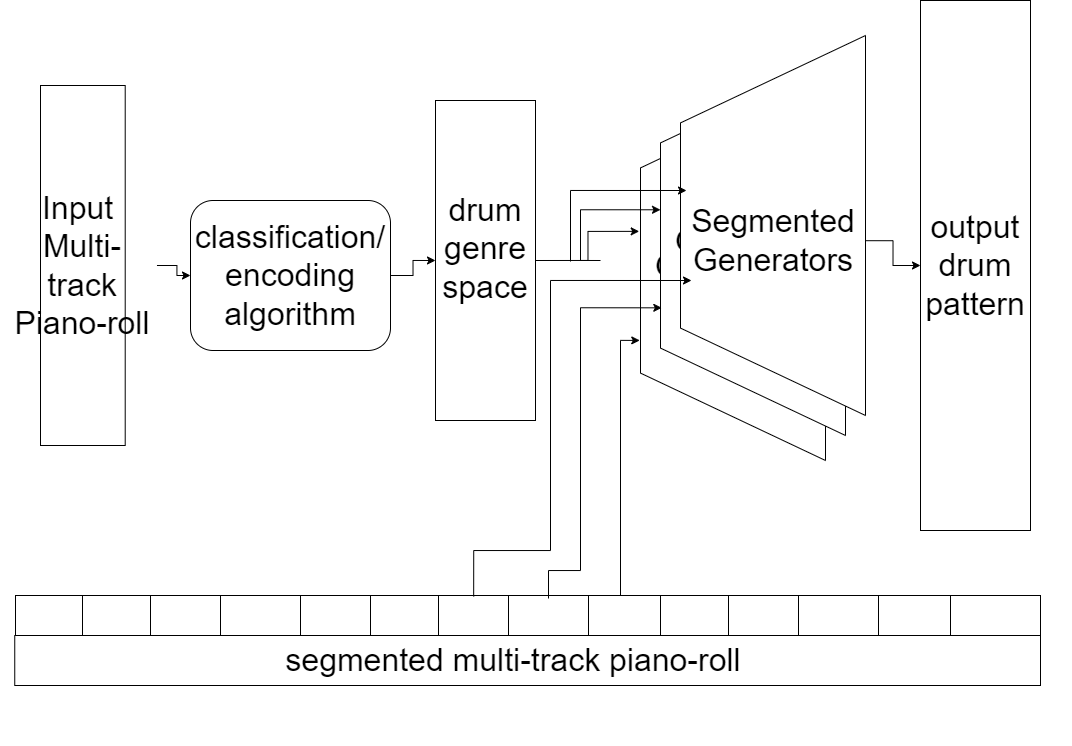
\includegraphics[width=3in]{image/proposal_architecture}
        \caption{General Pipeline the model}
        \label{fig:archie}
    \end{figure}
\end{par}

\begin{par}
    \par \hspace{15pt} Figure 1 shows the general pipeline of the proposed model. The model can be split into 2 parts: classification and generation. The output (before the last layer) of the classifier is fed into the generator as global induction. After that, the generator and the discriminator work together as a Generative Adversarial Network (GAN) to produce the final output.
\end{par}